% Chapter Template

\chapter{Mejoras futuras y Conclusiones} % Main chapter title

\label{ChapterX} % Change X to a consecutive number; for referencing this chapter elsewhere, use \ref{ChapterX}

\lhead{Capitulo 4. \emph{Conclusiones}} % Change X to a consecutive number; this is for the header on each page - perhaps a shortened title

%----------------------------------------------------------------------------------------
%	SECTION 1
%----------------------------------------------------------------------------------------

\section{Mejoras futuras}

Son muchas las mejoras que pueden hacerse en MODI, el diseño es un cuento de nunca acabar. En esta primera versión se priorizaron los requerimientos para construir un enjambre, dejando un poco de lado algunos aspectos que pueden ser importantes pero que no son parte fundamental del proyecto.

A continuación se explican algunas de las mejoras que pueden realizarse y como implementarlas.


%-----------------------------------
%	SUBSECTION 1
%-----------------------------------
\subsection{Encoders}
Una de las características claves de MODI es que hace uso de un tag fiducial, para poder tener información de la posición y orientación de cada robot. Con esto es posible controlar la navegación del robot, pero debido al roce o deslizamiento de las ruedas, se pueden mover diferente a lo esperado, provocando un error en la posición final. Si se necesita tener un control más fino sobre cada uno de los motores es fundamental incluir encoders en las ruedas. Por los motores que se tiene, se sugiere usar los enconders Pololu \footnote{http://www.pololu.com/catalog/product/1217}. Esta mejora no se implementó ya que implica modificar el PCB MODI para poder conectar los encoders al micro controlador Arduino.

%-----------------------------------
%	SUBSECTION 2
%-----------------------------------
\subsection{Cables incrustados y Soporte motor}
Es ideal que el mismo chasis del robot pueda contener las conexiones eléctricas y así reducir aún más la dificultad de ensamblado. Es por esto que se propuso un diseño con pequeños canales para incrustar los cables de los motores y que, además permite usar pins en los extremos que sirven para conectar eléctricamente los motores. Se puede ver en la Figura \ref{fig:Cables incrustados} esta idea, junto con una versión mejorada del soporte para los motores Pololu, que son motores ampliamente usados en robotica.

\begin{figure}[htbp]
	\centering
		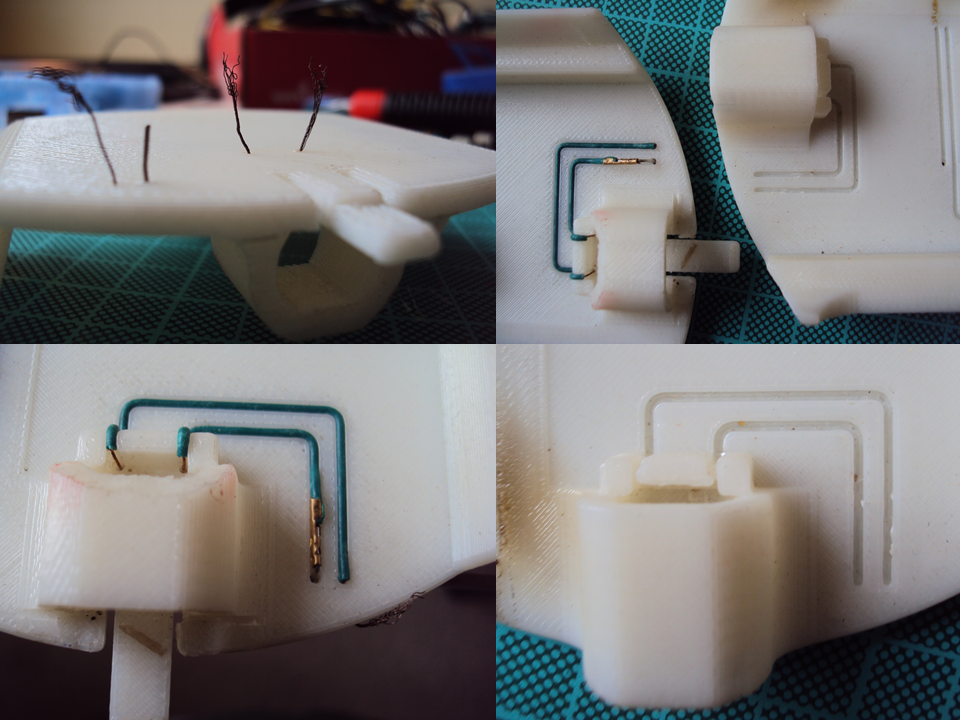
\includegraphics[width=\textwidth]{./Pictures/wires.png}
		\rule{35em}{0.5pt}
	\caption[Cables incrustados y Soporte motor]{Diseño propuesto por Dr. Pablo Prieto para optimizar el cableado eléctrico en el chasis de MODI. También se puede ver otra versión del Soporte motor, que incluye una pestaña que afirma al motor.}
	\label{fig:Cables incrustados}
\end{figure}	






%-----------------------------------
%	SUBSECTION 4
%-----------------------------------

\subsection{Una PCB para todo}

Para simplificar las conexiones del robot es necesario diseñar un nuevo PCB que incluya: Arduino, Driver motores y socket XBee, componentes electrónicos de MODI en Figura \ref{fig:compELO}. Esto debido a que demanda cierto tiempo tener que hacer los conectores necesarios para que se comuniquen entre sí. Tener este PCB implica bajar los costos de fabricación ya que es una sola PCB que se manda a fabricar, en vez de comprar tres en el mercado. Cabe destacar que esto debe ser un trabajo relativamente simple ya que todas las placas utilizadas son Open Source, lo que implica que sus archivos de diseño se encuentran completamente libre para su distribución, estudio, modificación y uso.


%-----------------------------------
%	SUBSECTION 2
%-----------------------------------

\subsection{Módulo de carga inalámbrica}
La elección de tener un Lipo Rider Pro en el robot en parte considera el uso de diversas formas de carga de energía. De forma simple se puede conectar un panel solar con conector JST 2.0, y en este mismo conector se puede poner un módulo de carga inalámbrica como el que vende SeeedStudio \footnote{http://www.seeedstudio.com/depot/wireless-charging-module-p-1354.html}. Estas alternativas permiten tener un setup de robots funcionando ininterrumpidamente ya que no es necesario intervenir los robots para cargar sus baterías. 


%----------------------------------------------------------------------------------------
%	SECTION 2
%----------------------------------------------------------------------------------------

\section{Conclusiones}
Diseñar un robot es una hermosa misión que implica desarrollar e integrar habilidades en varias áreas. Por lo mismo es necesario tener un equipo multidisciplinario que pueda abordar el problema desde distintas perspectivas. Para este trabajo fue fundamental contar con visiones expertas en robótica, diseño y biología-electrónica para hacer que MODI sea un gran proyecto que en un futuro pueda involucrar a mucha gente.

Con el equipo de trabajo armado los desafíos son adaptarse a la realidad nacional, donde se tienen menos recursos, tanto monetarios como de \textit{materias primas electrónicas}. Por esto es necesario lograr  hacer pruebas a pequeña escala para tomar decisiones en el diseño. Una herramienta fundamental para hacer pruebas a pequeña escala son las impresoras 3D que permiten en un día probar varios modelos distintos y hacer pruebas que no implican grandes pérdidas. Además de las impresoras 3D, con acceso a una Router CNC y un laboratorio básico de electrónica se puede hacer un producto que puede competir en el mercado.

Otras herramientas importantes en este trabajo son las tecnologías Open Source, que más bien es una filosofía donde se entrega de manera libre a la comunidad trabajo de gran calidad para que sea \textit{utilizado, modificado y compartido}. Muchos de los elementos importantes de MODI son Open Source, lo que implica que MODI también es un proyecto Open. Gracias a que se incluyeron estas tecnologías se pudo reducir el tiempo de desarrollo drásticamente.

MODI como robot es simple, tan simple que si no se tienen aplicaciones concretas el proyecto puede diluirse. Es importante hacer difusión del proyecto y en especial trabajar con áreas que estén algo más alejadas de la electrónica, que son las más beneficiadas con MODI ya que al tener una curva de aprendizaje rápida, permite enfocarse sólo en la tarea fundamental y dejar de lado los aspectos técnicos que implican construir un robot. Se recomienda que gente del área de la zoología, biología, visión, psicología, educación, informática, por nombrar algunas, se les capacite y facilite el acceso a esta plataforma que puede ayudar a desentrañar aspectos claves de nuestra naturaleza.

Un ejemplo de aplicación en otras áreas es el uso de este robot en educación. Muchos de los elementos incluidos en MODI, ya sea software o hardware, son grandes herramientas que pueden ser útiles para resolver otros desafíos tecnológicos como hacer uso de sensores inalámbricos o trabajar con energía solar, que gracias a la simplicidad del proyecto quedan expuesto de manera clara y modular. Es por esto que MODI es ideal como robot para introducirse en la robótica, permitiendo al usuario de manera libre estudiar todas sus características en la medida que lo necesite. De lograrse esto, se tendría un gran impacto educacional en Chile ya que MODI podrá ser la puerta de entrada para introducir fácilmente la robótica en el sistema educacional chileno.